\section{Parte II}

\subsection{Problema}

\par Se solicita  utilizar cualquier método o técnica numérica para resolver la ecuación diferencial parcial de Cromatografía de Membrana. La cromatografía es un método de separación en cual los componentes a ser separados se distribuyen en dos fases: una fija (fase estacionaria) y otra que se mueve en una determinada dirección (fase móvil). Las ventajas de utilizar una membrana para el proceso de separación es una transferencia de masa rápida, el flujo a través de la membrana no está limitado por la caída de presión.

\begin{figure}[!ht]
	\centering
	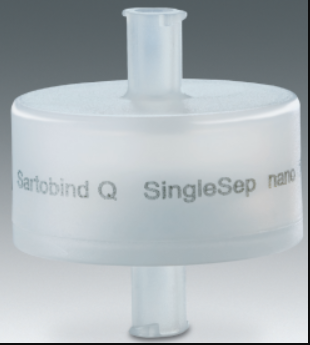
\includegraphics[scale=0.7]{Imagenes/membrana.png}
	\caption{Figura de la membrana}
	\label{fig:ej}
\end{figure}

Se modela utilizando el balance de proteínas en la fase móvil (5). La ecuación diferencial parcial para cada proteína (i=1....N) en la fase móvil. Donde $Cb_{i}$ es la concentración en el fluido y $Cb^*_{i}$ la concentración de proteína en la membrana

\begin{equation}
\begin{split}
       -D_{bi}\cdot\frac{\partial^2 Cb_{i}}{\partial z^2}+\frac{\partial Cb_{i}}{\partial z}+\frac{\partial Cb_{i}}{\partial t}+ \varepsilon(Cb_{i}-Cb^*_{i}) = 0
\end{split}
\end{equation}

\par Independiente del método utilizado para resolver la ecuación, la cromatografía de elución se lleva a cabo realizando los pasos de: inyección de la muestra, lavado de columna y
elución. Con esto se deben obtener las curvas de elución y modulación de cromatografía, junto con una gráfica en 3 dimensiones que muestre la difusión tiempo-espacio. Además, para el método utilizado debe entregar los errores (eficacia) y eficiencia (costo computacional) de este.

\subsection{Solución}

\subsubsection{Método de Diferencias Finitas}

\par  Para obtener resolver la ecuación anterior, se utiliza el método de diferencias finitas sobre ecuaciones diferenciales parciales, para esto se deben establecer las condiciones de frontera las cuales son:

\begin{itemize}
	\item Cb(z,0) = 0   $0 < z < L$;  L: Largo de la columna
	\item Cb(L,t) = 0  $0< t < tmax$; donde el tmax equivale al largo t de la matriz
	\item Cb(0,t) = funcion pulso; cuando $t < tinyeccion$; t = 2 y cuando $t > tinyeccion$, t = 0
\end{itemize}

Lo primero que se debe hacer para una ecuación utilizando diferencias finitas es discretizar la ecuación. Para la discretización del dominio se crea una matriz de $n x m$ donde n seria las veces que divide la columna (nz) y m el tiempo aproximado que nosotros le damos a que se realiza la cromatografía. Una forma de representarlo sería:

\begin{figure}[!ht]
	\centering
	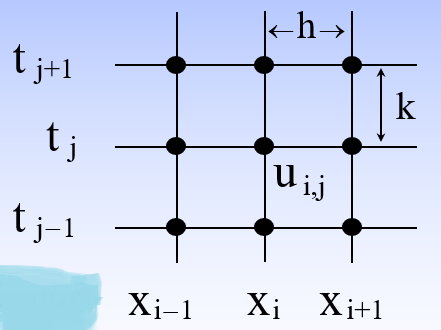
\includegraphics[scale=0.6]{Imagenes/matriz.png}
	\caption{Forma de representar la matriz}
	\label{fig:ej}
\end{figure}

\par Donde $u_{i,j}$ seria el $Cb_{i}$ de la ecuación, h y k serian dz y dt respectivamente. Y x es lo mismo que z. Para elegir los puntos en los cuales calcularemos la solución aproximada de la EDP. Al discretizar los términos tambien dividimos dz/dt obteniendo el valor B y A = (1-B), obtenemos (6):

\begin{equation}
\begin{split}
    \frac{1}{PE}\cdot\frac{Cb_{i-1,j}-2Cb_{i,j}+Cb_{i+1,j}}{h^2} + B\cdot Cb_{i-1,j-1} + A\cdot Cb_{i,j-1}
\end{split}
\end{equation}


\subsubsection{Elución y Modulación}

\par Antes de explicar la graficar se debe indicar que los parámetros nz y tiempo son muy limitados, por lo realizado en este laboratorio nz no puede ser inferior a 15 o superior a 22 y el tiempo en el cual se efectúa debe estar entre 90 y 110, para que se obtengan las curvas de elución y modulación. 

\par Para obtener la curva de elución, debe graficar según los resultados obtenidos en el último z antes de llegar al largo L de la columna (Ya que en L, el tiempo es 0) . Para la curva de modulación se debe guardar los valores de sal desde el proceso de inyección, lavado hasta el proceso de elución (se especifica mejor en el código).

\subsection{Resultados}

\par En esta sección entregaremos cada uno de los resultados obtenidos al aplicar el método de diferencias finitas en matlab.

\subsubsection{Primera prueba}

\par Como se mencionó anteriormente, el tiempo y el z debe ser los mencionados para que sea estable y se pueda obtener una gráfica entendible. Para la primera prueba se usó una matriz de ancho nz = 20 y un t = 100. Obteniendo los siguientes resultados:

\begin{figure}[!ht]
	\centering
	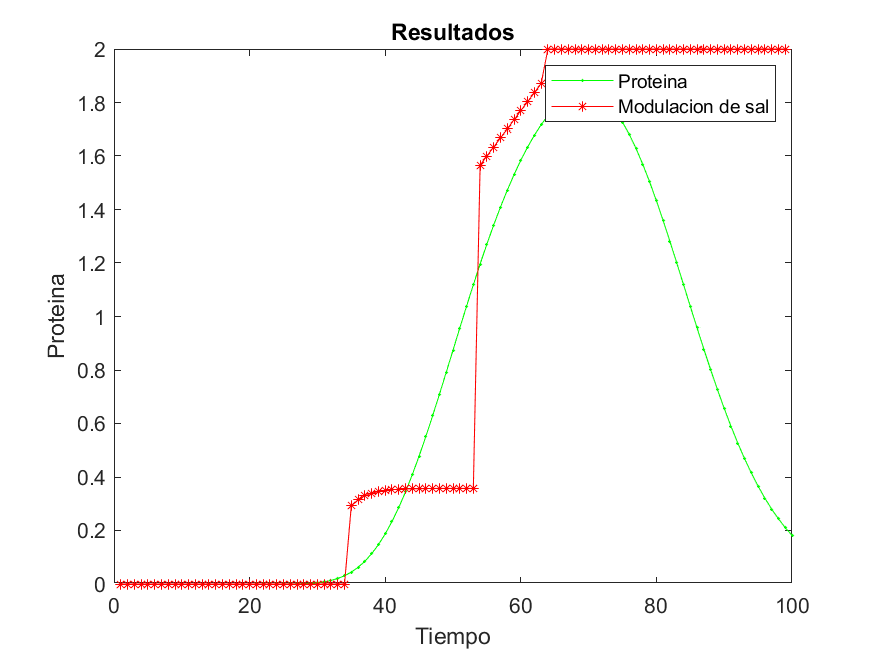
\includegraphics[scale=0.6]{Imagenes/resultado1.png}
	\caption{Resultado de las curvas de elución (verde) y modulación (rojo)}
	\label{fig:ej}
\end{figure}

\par Además de obtener la difusión tiempo y espacio para $Cb_{i}$

\begin{figure}[!ht]
	\centering
	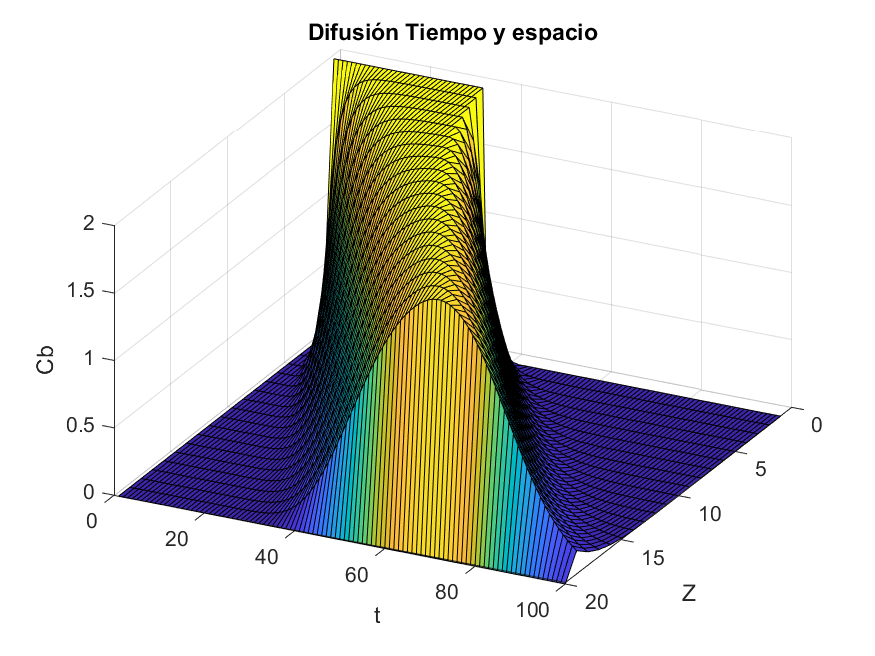
\includegraphics[scale=0.7]{Imagenes/grafico3d.png}
	\caption{Gráfico de difusión en tiempo-espacio}
	\label{fig:ej}
\end{figure}

\par Para el método utilizado de diferencias finitas se agregaron los indicadores de eficacia (error) y eficiencia (costo computacional). El error es la resta del mínimo valor con el anterior y el ultimo digito es divido por la cantidad de dígitos, el costo computacional es la cantidad de operaciones que debe realizar el computador (+,-,x,/).

\begin{table}[htp]
	\centering
	\begin{tabular}{ |c|c|c|}
		\hline
		\textbf{Método} & \textbf{Error} & \textbf{Costo Computacional}  \\
		\hline
		Direncias Finitas & 0.0354 &  23.253 \\
		\hline
	\end{tabular}
	\caption{Tabla de resultados para la primera prueba}
	\label{tab:tab3}
\end{table}

\newpage

\subsubsection{Segunda Prueba}

\par Para la segunda prueba el nz seleccionado fue 22 y para el tiempo fue 120, con lo cual se obtuvieton los siguientes resultados.

\begin{figure}[!ht]
	\centering
	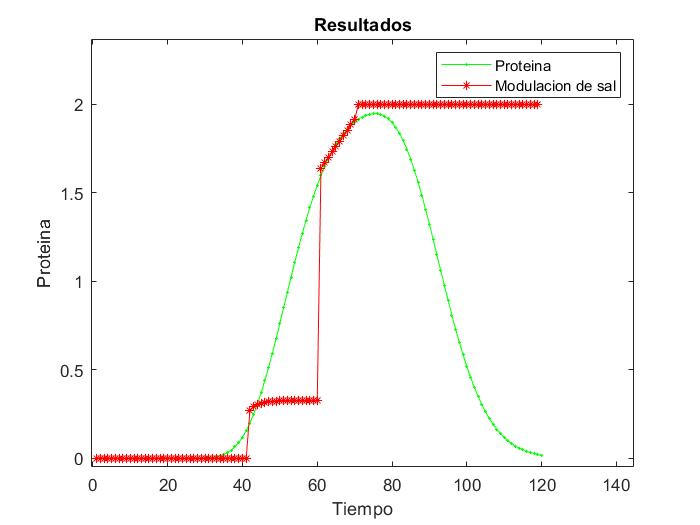
\includegraphics[scale=0.4]{Imagenes/graficoem2.jpg}
	\caption{Resultado de las curvas de elución (verde) y modulación (rojo)}
	\label{fig:ej}
\end{figure}

\newpage

\par Además de obtener la difusión tiempo y espacio para $Cb_{i}$

\begin{figure}[!ht]
	\centering
	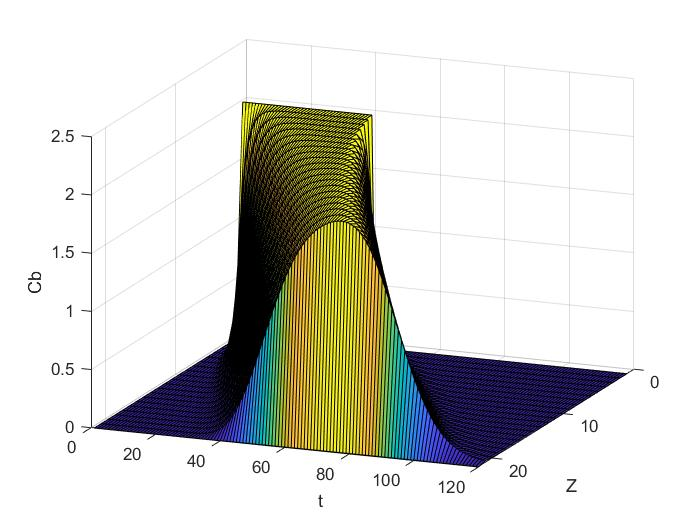
\includegraphics[scale=0.6]{Imagenes/grafico3d2.jpg}
	\caption{Gráfico de difusión en tiempo-espacio}
	\label{fig:ej}
\end{figure} 

\par Para el método utilizado de diferencias finitas se agregaron los indicadores de eficacia (error) y eficiencia (costo computacional).

\begin{table}[htp]
	\centering
	\begin{tabular}{ |c|c|c|}
		\hline
		\textbf{Método} & \textbf{Error} & \textbf{Costo Computacional}  \\
		\hline
		Direncias Finitas & 0.0265 &  31.057 \\
		\hline
	\end{tabular}
	\caption{Tabla de resultados para la primera prueba}
	\label{tab:tab3}
\end{table}



















